\chapter{Billedkomprimering med diskret cosinustransformation}

\subsection{Den diskrete fouriertransformation}
Inden signalbehandling er den diskrete Fouriertransformation (DFT) et kendt værktøj. Transformationen er en lineær transformation, som udtrykker et signal på bølgeform ved sinus- og cosinusfunktioner\citep{thefouriertransform}. De fleste signaler er på bølgeform og kan derfor beskrives ved sinus- og cosinusfunktioner gennem DFT.\\
Signaler kan altså beskrives i to domæner
\begin{itemize}
	\item{\textit{Tidsdomænet}\\
	Signalet beskrives ved funktionsværdier til tiden $t$, $f(t)$.}
	\item{\textit{Frekvensdomænet}\\
	Signalet beskrives ved amplitude og fase for en frekvensfunktion.}
\end{itemize}
Regneoperationer i tidsdomænet har tilsvarende regneoperationer i frekvensdomænet, som ofte er beregningsmæssigt simplere \citep{nbtwiki}. Af denne grund bruges den diskrete Fouriertransformation til signalbehandling.\\
Transformationen har desuden den egenskab, at den energikomprimerer signalet, som behandles. Energikomprimering betegner en transformations evne til at udtrykke mange signalværdier med høje korrelation i domænet som færre koefficienter med lav korrelation i kodomænet \citep{smcnus_energy}. Koefficienterne i frekvensdomænet er koefficienterne hvorved basisfunktionerne i transformationen optræder i signalet i tidsdomænet - høje koefficienter viser en høj optræden af den tilhørende basisfunktion, mens lave koefficienter viser en lav optræden af den tilhørende basisfunktion.

Når DFT udtrykker korrelerede signalværdier som ukorrelerede koefficienter i frekvensdomænet, betyder det også at transformationen ikke formår at lave energikomprimering i høj grad, hvis signalværdierne er ukorrelerede. Dette betyder at, hvis man ønsker høj energikomprimering, DFT kun skal bruges på signaler, som består af korrelerede værdier.

I billedkomprimering er man, som tidligere beskrevet, interesseret i at udtrykke et billede ved færre værdier, da det derfor kan udtrykkes simplere. DFT kan være et værktøj til dette. DFT fungerer da også bedst på sginaler, som består af korrelerede værdier, og det gør netop et billede. DFT kan altså bruges til billedkomprimering.

Det viser sig imidlertid, at der findes et bedre værktøj til tranformation af korrelerede signalværdier til ukorrelerede koefficienter. Transformationen kaldes den diskrete cosinustransformation (DCT), og er udledt fra DFT. Udledningen ses i appendix \vref{DCT_udledning}.\\
DCT udmærker sig inden for billedbehandling på flere områder i forhold til DFT
\begin{enumerate}
	\item{\textit{Energikomprimering}\\
	Den diskrete cosinustransformation opnår højere energikomprimering end DFT \citep{smcnus_energy}. Dette er ønskværdigt inden for billedkomprimering, da man ønsker at udtrykke meget information ved få koefficienter.}
	\item{\textit{Reelle tal}\\
	DFT benytter både reelle og komplekse koefficienter til at beskrive et signal i frekvænsdomænet. DCT benytter udlukkende reelle tal. \fixme{Hvorfor er vi ikke interesserede i komplekse tal?}}
	\item{textit{Hastighed}\\
	DFT benytter sig af dobbelt så mange basisfunktioner og dermed koefficienter som DCT til at beskrive et signal. Da man i billedkomprimering ønsker så få koefficienter som muligt, er DCT smartere.}
\end{enumerate}

\subsection{JPEG}
Joint Photographic Experts Group udgav i 1992 den første JPEG-standard, som komprimerede og dekomprimerede billeder efter en bestemt algoritme. Et program, som kan gøre dette kaldes en codec. Standarden er open source og er siden 1992 blevet forbedret flere gange. Vi vil her beskæftige os med en simpel og tidlig version.\\
JPEG gør brug af fire skridt i sin algoritme for at komprimere et billede fra dets fulde størrelse til en fil af mindre størrelse. Den inverse algoritme bruges til at dekomprimere en .jpg-fil til et billede. Da JPEG er en komprimeringsalgoritme med tab, vil det dekomprimerede billede kun være en efterligning af det originale. \citep{whydomath_basic}.\\
De fire skridt, som forklares nærmere i senere afsnit, ser ud som følger
\begin{enumerate}
	\item{\textit{Forbehandling af billede}\\
	Forbehandlingen indebærer at dele billedet op i kvadratiske blokke af 64 pixels. Dette gøres for at gøre den videre behandling af billedet med den diskrete cosinustransformation mere effektiv.}
	\item{\textit{Diskret cosinus transformation}\\
	Den diskrete cosinustransformation energikomprimerer billedet ved at udtrykke korrelerede signalværdier som dekorrelerede koefficienter i frekvensdomænet - billedet energikomprimeres.}
	\item{\textit{Kvantisering}\\
	Kvantiseringen fjerner mindre vigtige informationer om billedet ved at fjerne de dekorrelerede koefficienter som ikke er vigtige i forhold til de korrelerede signalværdier.. Dette skridt er hvad der gør algoritmen til én med tab.}
	\item{\textit{Entropikodning}\\
	Dette skridt opstiller en statistisk model over de kvantiserede koefficienter og koder dem i strenge af 0- og 1-taller, som kan gemmes effektivt i en fil, som er mindre end den oprindelige billedfil.}
\end{enumerate}

For at forstå hvorfor og hvordan algoritmen virker er det nødvendigt at forstå den diskrete cosinustransformation. Derfor vil dette skridt blive forklaret først.

\subsection{Diskret Cosinustransformation}\label{sec:DCT}
En diskret cosinustransformation er en lineær transformation som afbilder en \textit{n}-dimensionel vektor fra domænet $\mathbb{R}^n$ til kodomænet $\mathbb{R}^n$. Basisvektorerne i transformationen udledes fra cosinusfunktioner med foreskellige frekvenser. Som følge af dette bliver den \textit{n}-dimensionelle vektor afbildet ind i frekvensdomænet - den udtrykkes som en sum af cosinusfunktioner med forskellige frekvenser. Et eksempel på en funktion udtrykt ved bølgefunktioner ses på figur \vref{fig:sumafboelger}. Der ses bort fra x- og y-aksen, som ikke nødvendigvis passer på vores beregninger.

DCT'en bruges i udstrakt grad i signalbehandling på grund af dens høje energikomprimering. DCT'en kan altså komprimere meget signalværdi ned til få værdier i frekvensdomænet og dermed udtrykke signalværdier med stor korrelation som koeffiencienter med lav eller ingen korrelation. Transformationen fungerer dog bedst, når signalværdierne som transformeres har en hvis korrelation - hvis dette ikke er tilfældet, vil der ikke blive opnået gode resultater med transformationen \citep{smcnus_energy}.

DCT er imidlertid ikke den eneste transformation, som kan dekorrelere signalværdier. En anden kendt transformation er Karhunen-Loeve transformationen. Denne transformation transformerer, som cosinustransformationen, også korrelerede koefficienter til dekorrelerede koefficienter. Karhunen-Loeve udmærker sig ved at tilpasse sig hvordan signalet ser ud, for således at kunne energikomprimere meget effektivt - transformationen afhænger altså af signalet. Dette gør transformationen i stand til at lave den mest effektive energikomprimering \citep{lokminglui_DCT}. Det er imidlertid ikke tidsmæssigt effektivt, at skulle komponere en ny transformation hver gang et nyt signal behandles og derfor bruges den diskrete cosinustransformation. Denne har en algoritme, som genererer en generel transformation \citep{electronic_engineering}.

Den diskrete cosinustransformation er desuden udledt fra den diskrete Fouriertransformation (DFT), som også transformerer et digitalt signal i diskret tid fra tidsdomænet til frekvensdomænet. Den diskrete cosinusfunktion udmærket sig dog i forhold til Fouriertransformationen ved at have højere energikomprimering, hvilket er præcis hvad vi har brug for til billedkomprimering. Desuden formår den at udtrykke de korrelerede signalværdier ved færre ukorrelerede frekvensværdier end Fouriertransformationen \citep{smcnus_energy}.

Da DCT er en lineær transformation og fungerer godt, når signalet, som skal behandles, har stor korrelation, kan den bruges i billedbehandling til at energikomprimere digitale billeder, som netop er matricer, og som vi antager har stor korrelation mellem nærliggende pixels.

\begin{figure}[htbp]
\centering
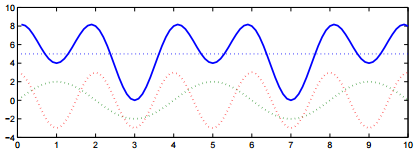
\includegraphics[width=0.5\textwidth]{Billeder/sumafboelger.png}
\caption{Funktion (blå) og bølgefunktioner (stiplede) brugt til at udtrykke funktionen.}
\label{fig:sumafboelger}
\end{figure}

Den diskrete cosinustransformation, som kan udledes fra den diskrete Fouriertransformation, kan transformere i både én og to dimensioner. I denne opgave benyttes den todimensionelle. I ligning \vref{eq:DCTeq} ses den todimensionelle n-punkt diskrete cosinustransformation, som transformerer en $n \times n$-matrix til en $n \times n$-matrix indeholdende dekorrelerede koeffecienter \citep{guillermo_sapiro}. Vi vil fremover kalde matricen, vi transformerer for A. 
\begin{equation}
T^{II}_{(i,j)}=\sum\limits_{x=0}^{n-1} \sum\limits_{y=0}^{n-1} f(x,y) \cdot \alpha(i) \cdot \alpha(j) \cdot \cos\left(\frac{(2x+1)\cdot i \cdot \pi}{2n}\right) \cdot \cos\left(\frac{(2y+1)\cdot j \cdot \pi}{2n}\right)
\label{eq:DCTeq}
\end{equation}
Hvor
\begin{itemize}
	\item{$T^{II}_{(i,j)}=$ indgang $(i,j)$ i den transformerede matrix ved DCT}
	\item{$f(x,y)=$ indgang $(x,y)$ i A}
	\item{$n=$ matricens størrelse $n\times n$}
	\item{$\alpha(i)=\alpha(j)=\begin{cases}
						\sqrt{\frac{1}{n}} \ hvis \ i = 0\\
						\sqrt{\frac{2}{n}} \ hvis \ i \neq 0
					\end{cases}$}
\end{itemize}
Det er værd at bemærke at indgangene i matricen går fra $(0,0)$ til $(n-1,n-1)$ i en $n \times n$ matrix.\\
$\alpha(i)$  og $\alpha(j)$ er funktioner, som sørger for at normalisere signalet. Transformationen tilpasser sig størrelsen af matricen og producerer derfor normaliserede koefficienter. Dette er vigtigt i data- og signalbehandling, da dette kræver at dataerne er på samme form og enheder \citep{normalization}.

Ligning \vref{eq:DCTeq} bruges i denne opgave ikke til at beregne de transformerede koefficienter, da det beregningsmæssigt ikke er effektivt. Til dette bruges i stedet cosinustransformationen på matrixform, hvilket uddybes senere i dette afsnit. Ligning \vref{eq:DCTeq} er imidlertid god til at illustrere princippet bag transformationen, da det er tydeligt hvordan cosinusfunktioner indgår i transformationen. Dette vil vi se nærmere på nu.

Det ses af ligning \vref{eq:DCTeq} at hver transformeret indgang er summen af produktet af de 64 indgange i A og en koefficient fra en cosinusfunktion. For hver række $f(x,y)$ holdes $x$ konstant gennem de 8 søjler hvor $y$ går fra $0-7$. Dette giver koefficienter der alle ligger på en cosinuskurve. Hver gang en ny række $x$ påbegyndes, ændres amplituden af cosinusbølgen, som koefficienterne ligger på.\\
Når en ny transformeret indgang $T_{(i,j)}$ beregnes, ændres $i$ og/eller $j$ og frekvensen af cosinusfunktionerne i transformen bliver højere. Altså bliver hver transformeret indgang et unikt aftryk af forskelligt svingene cosinusfunktioner og værdierne i billedmatricen A.

For at illustrere princippet bag de skiftende amplituder og frekvenser af cosinusbølgerne, som koefficienterne ligger på er to sæt af grafer for cosinustransformationen tegnet i figurerne \vref{fig:frekeksu1v1} og  \vref{fig:frekeksu1v2}. Disse er tegnet ved brug af transformationen i ligning \vref{eq:DCTeq} for henholdsvis $T(1,1)$ og $T(1,2)$ og for $n=8$. For hver af funktionerne fremkommer 8 bølger og på hver af disse ligger de 8 koefficienter ligeligt fordelt. På figur \vref{fig:cosko} ses de 8 punkter på én af bølgerne for $T(0,0)$.

\begin{figure}[!h]
\begin{minipage}[b]{0.5\linewidth}
\centering
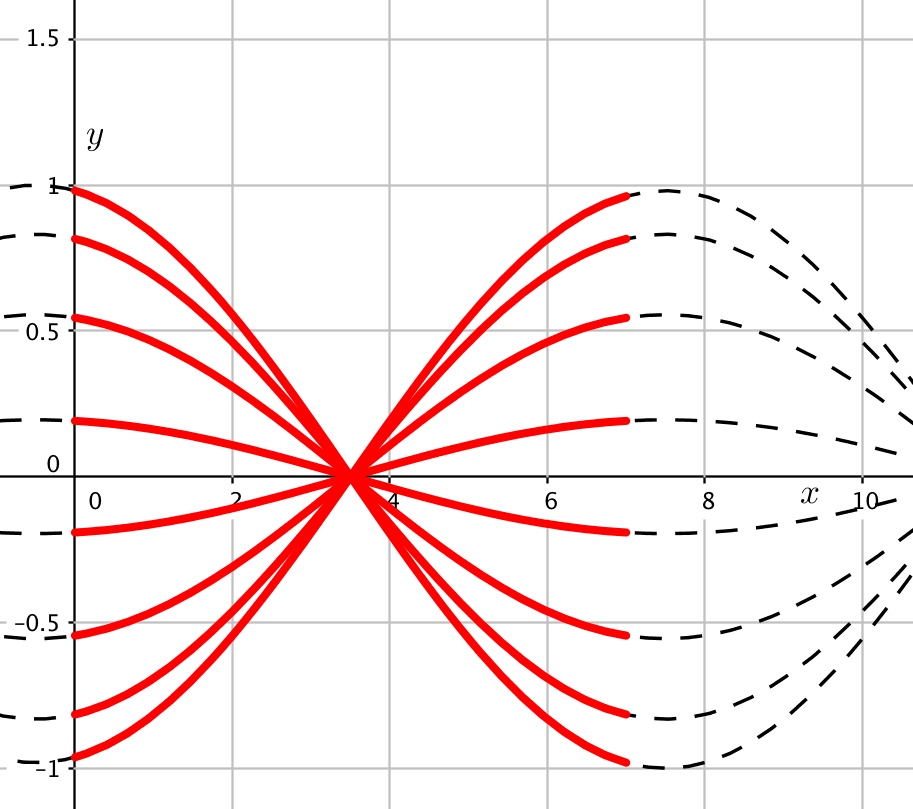
\includegraphics[width=0.5\textwidth]{Billeder/Frekvens-eksempelu1v1.png}
\caption{Bølger for hver række for $T(1,1)$ tegnet ved brug af ligning \vref{eq:DCTeq}. På hver af disse bølger ligger 8 ligeligt fordelte koefficienter, som multipliceres med signalværdierne.}
\label{fig:frekeksu1v1}
\end{minipage}
\hspace{0.5cm}
\begin{minipage}[b]{0.5\linewidth}
\centering
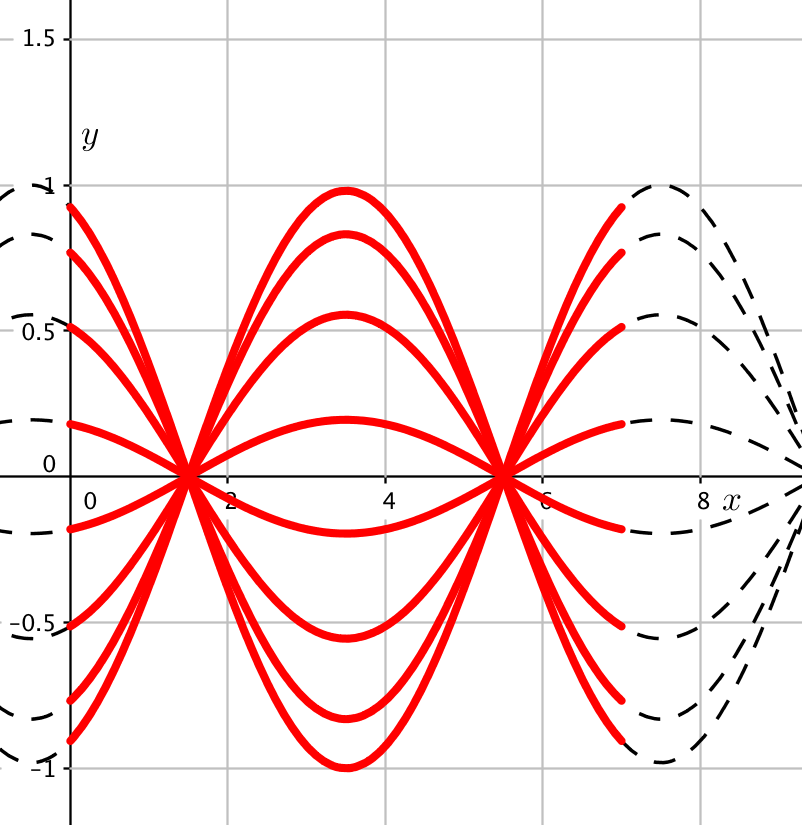
\includegraphics[width=0.5\textwidth]{Billeder/Frekvens-eksempelu1v2.png}
\caption{Bølger for hver række for $T(1,2)$.}
\label{fig:frekeksu1v2}
\end{minipage}
\end{figure}

\begin{figure}[htbp]
\centering
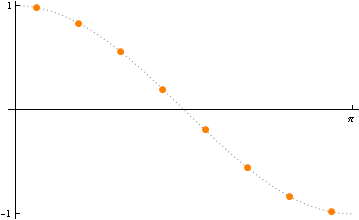
\includegraphics[width=0.5\textwidth]{Billeder/coskoefficienter.png}
\caption{Koefficienterne for $T(1,1)$ og $f(0,y)$ afmærket som punkter på en cosinusbølge.}
\label{fig:cosko}
\end{figure}

Det ses desuden på figur \vref{fig:cosko} at koefficienterne tilsammen har en sum = 0. Der er altså lige mange positive og negative koefficienter i alle bølgerne med untagelse af den første, som udelukkende består af koefficienten $\frac{\sqrt{2}}{2}$.\\
At hele den første række kun indeholder positive indgange bidrager til energikomprimeringen. Hvis A indeholder lignende værdier vil indgang $(0,0)$ have stor numerisk værdi. Derfor kan en stor del af informationerne koncentreres i den ene indgang. På samme måde vil resultatet af at prikke en konstant vektor med en hvilken som helst samling af koefficenter fra en cosinusbølge beregnet ved $i=1,...,7$ blive lig 0. Resultatet af at prikke en hvilken som helst næsten konstant vektor med koefficienterne vil blive tæt på eller lig 0 \citep{whydomath_dct}.\\
Koefficienten i indgang $(0,0)$ kaldes for DC koefficienten for Direct Current. De resterende 63 koefficienter kaldes for AC koefficienter for Alternating Current. Navnene stammer fra transformationens historiske brug i analyse af elektriske kredsløb. Navnene refererer til basisfunktionerne i transformationen, som for DC koefficienten er konstant søm jævnstrøm, men de oscillerer som vekselstrøm for de resterende koefficienter  \citep{lokminglui_DCT}.

De transformerede koefficienter udtrykker bestemte mønstre i signalet. Mønstrene for hver koefficient ses på figur \vref{fig:frekvens_matrix}, hvor bølgetoppene og -dalene i basisfunktionerne (og dermed negative og positive koefficienter) er henholdsvis sorte og hvide. Denne figur illustrerer hvordan transformationen behandler forskellige slags mønstre i signalet - mønstre som ligner signalet vil have høje koefficienter. Bemærk at DC koefficienten er koefficient for et ensfarvet mønster eller signal.
\begin{figure}[htbp]
\centering
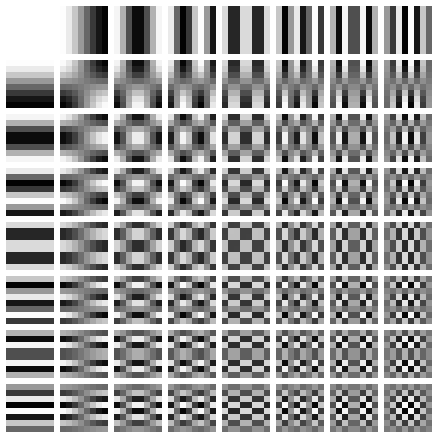
\includegraphics[width=0.5\textwidth]{billeder/frekvensmatrix.png}
\caption{Repræsentation af de 64 forskellige basisfunktioner i cosinus transformationen af længde $n$. Mønstrene hører til koefficienterne, som fås ved transformation af et signal. Koefficienternes størrelse fortæller hvor meget det tilhørende mønster optræder i signalet.}
\label{fig:frekvens_matrix}
\end{figure}

Indgangene i den transformerede matrix er koefficienterne hvorved disse mønstre er repræsenteret i signalet. Altså kan signalet genskabes ved en lineær kombination af disse mønstre.

I dette projekt udføres beregninger og dermed også transformationen i Python. Til dette er det beregningsmæssigt nemmere og hurtigere at regne med DCT'en på matrixform. Ligning \ref{eq:DCTmatrixform} er den diskrete cosinustransformation af længde $n$ og producerer indgang $(i,j)$ i en matrix af størrelse $n \times n$ som kan bruges på samme måde som transformationen i \vref{eq:DCTeq}. Matricerne indeholder de tidligere omtalte koefficienter som bl.a. ses på figur \ref{fig:cosko}.
\begin{align}
	y_{(i,j)} = C(i) \sqrt{\frac{2}{n}} \cos\left(\frac{(2 \cdot j-1) \cdot (i-1)\pi}{2n}\right)
\label{eq:DCTmatrixform}
\end{align}
Hvor
\begin{itemize}
		\item{$C(i)= \begin{cases}
			\frac{1}{\sqrt{2}} \ hvis \ i = 1\\
			1\ \ \ hvis \ i \neq 1
		\end{cases}
		$}
		\item{$y_{(i,j)}=$ indgang $(i,j)$}
		\item{$n =$ matricens dimensioner n$\times$n}
\end{itemize}
Matricen beregnet ved formel \vref{eq:DCTmatrixform} hvor $n=8$ ses på figur \ref{eq:DCTmatrix}. I beregningerne bruges desuden den transponerede matrix, som ses på figur \Vref{eq:DCTmatrixT}.
\begin{equation}
U=\frac{1}{2}
\begin{bmatrix}
	\frac{\sqrt{2}}{2}	& \frac{\sqrt{2}}{2}		& \frac{\sqrt{2}}{2}		& \frac{\sqrt{2}}{2}		& \frac{\sqrt{2}}{2}		& \frac{\sqrt{2}}{2}		& \frac{\sqrt{2}}{2}		& \frac{\sqrt{2}}{2}		\\
	\cos(\frac{\pi}{16})		& \cos(\frac{3\pi}{16})	& \cos(\frac{5\pi}{16})	& \cos(\frac{7\pi}{16})	& \cos(\frac{9\pi}{16})	& \cos(\frac{11\pi}{16})	& \cos(\frac{13\pi}{16})	& \cos(\frac{15\pi}{16})		\\
	\cos(\frac{2\pi}{16})	& \cos(\frac{6\pi}{16})	& \cos(\frac{10\pi}{16})	& \cos(\frac{14\pi}{16})	& \cos(\frac{18\pi}{16})	& \cos(\frac{22\pi}{16})	& \cos(\frac{26\pi}{16})	& \cos(\frac{30\pi}{16})		\\
	\cos(\frac{3\pi}{16})	& \cos(\frac{9\pi}{16})	& \cos(\frac{15\pi}{16})	& \cos(\frac{21\pi}{16})	& \cos(\frac{27\pi}{16})	& \cos(\frac{33\pi}{16})	& \cos(\frac{39\pi}{16})	& \cos(\frac{45\pi}{16})		\\
	\cos(\frac{4\pi}{16})	& \cos(\frac{12\pi}{16})	& \cos(\frac{20\pi}{16})	& \cos(\frac{28\pi}{16})	& \cos(\frac{36\pi}{16})	& \cos(\frac{44\pi}{16})	& \cos(\frac{52\pi}{16})	& \cos(\frac{60\pi}{16})		\\
	\cos(\frac{5\pi}{16})	& \cos(\frac{15\pi}{16})	& \cos(\frac{25\pi}{16})	& \cos(\frac{35\pi}{16})	& \cos(\frac{45\pi}{16})	& \cos(\frac{55\pi}{16})	& \cos(\frac{65\pi}{16})	& \cos(\frac{75\pi}{16})		\\
	\cos(\frac{6\pi}{16})	& \cos(\frac{18\pi}{16})	& \cos(\frac{30\pi}{16})	& \cos(\frac{42\pi}{16})	& \cos(\frac{54\pi}{16})	& \cos(\frac{66\pi}{16})	& \cos(\frac{78\pi}{16})	& \cos(\frac{90\pi}{16})		\\
	\cos(\frac{7\pi}{16})	& \cos(\frac{21\pi}{16})	& \cos(\frac{35\pi}{16})	& \cos(\frac{49\pi}{16})	& \cos(\frac{63\pi}{16})	& \cos(\frac{77\pi}{16})	& \cos(\frac{91\pi}{16})	& \cos(\frac{105\pi}{16})	\\
\end{bmatrix}
\label{eq:DCTmatrix}
\end{equation}
\begin{equation}
U^T = \frac{1}{2}
\begin{bmatrix}
\frac{2}{\sqrt{2}} & \cos(\frac{\pi}{16}) & \cos(\frac{2 \cdot \pi}{16}) & \cos(\frac{3 \cdot \pi}{16}) & \cos(\frac{4 \cdot \pi}{16}) & \cos(\frac{5 \cdot \pi}{16}) & \cos(\frac{6 \cdot \pi}{16}) & \cos(\frac{7 \cdot \pi}{16}) \\
\frac{2}{\sqrt{2}} & \cos(\frac{3 \cdot \pi}{16}) & \cos(\frac{6 \cdot \pi}{16}) & \cos(\frac{9 \cdot \pi}{16}) & \cos(\frac{12 \cdot \pi}{16}) & \cos(\frac{15 \cdot \pi}{16}) & \cos(\frac{18 \cdot \pi}{16}) & \cos(\frac{21 \cdot \pi}{16}) \\
\frac{2}{\sqrt{2}} & \cos(\frac{5 \cdot \pi}{16}) & \cos(\frac{10 \cdot \pi}{16}) & \cos(\frac{15 \cdot \pi}{16}) & \cos(\frac{20 \cdot \pi}{16}) & \cos(\frac{25\cdot \pi}{16}) & \cos(\frac{30 \cdot \pi}{16}) & \cos(\frac{35 \cdot \pi}{16}) \\
\frac{2}{\sqrt{2}} & \cos(\frac{7 \cdot \pi}{16}) & \cos(\frac{14 \cdot \pi}{16}) & \cos(\frac{21 \cdot \pi}{16}) & \cos(\frac{28 \cdot \pi}{16}) & \cos(\frac{35 \cdot \pi}{16}) & \cos(\frac{42 \cdot \pi}{16}) & \cos(\frac{49 \cdot \pi}{16}) \\
\frac{2}{\sqrt{2}} & \cos(\frac{9 \cdot \pi}{16}) & \cos(\frac{18 \cdot \pi}{16}) & \cos(\frac{27 \cdot \pi}{16}) & \cos(\frac{36 \cdot \pi}{16}) & \cos(\frac{45 \cdot \pi}{16}) & \cos(\frac{54 \cdot \pi}{16}) & \cos(\frac{63 \cdot \pi}{16}) \\
\frac{2}{\sqrt{2}} & \cos(\frac{11 \cdot \pi}{16}) & \cos(\frac{22 \cdot \pi}{16}) & \cos(\frac{33 \cdot \pi}{16}) & \cos(\frac{44 \cdot \pi}{16}) & \cos(\frac{55 \cdot \pi}{16}) & \cos(\frac{66 \cdot \pi}{16}) & \cos(\frac{77 \cdot \pi}{16}) \\
\frac{2}{\sqrt{2}} & \cos(\frac{13 \cdot \pi}{16}) & \cos(\frac{26 \cdot \pi}{16}) & \cos(\frac{39 \cdot \pi}{16}) & \cos(\frac{52 \cdot \pi}{16}) & \cos(\frac{65 \cdot \pi}{16}) & \cos(\frac{78 \cdot \pi}{16}) & \cos(\frac{91 \cdot \pi}{16}) \\
\frac{2}{\sqrt{2}} & \cos(\frac{15 \cdot \pi}{16}) & \cos(\frac{30 \cdot \pi}{16}) & \cos(\frac{45 \cdot \pi}{16}) & \cos(\frac{60 \cdot \pi}{16}) & \cos(\frac{75 \cdot \pi}{16}) & \cos(\frac{90 \cdot \pi}{16}) & \cos(\frac{105 \cdot \pi}{16})
\end{bmatrix}
\label{eq:DCTmatrixT}
\end{equation}
Disse to matricer kan, som ligning \vref{eq:DCTeq} også bruges til at opnå transformationen. Her prikkes $U$ med $A$ og derefter prikkes dette resultat med $U^T$. Transformationen ses i ligning \vref{eq:DCTtrans}.
\begin{align}
B=U \cdot A \cdot U^T
\label{eq:DCTtrans}
\end{align}
Hvor
\begin{itemize}
	\item $B$ = den transformerede matrix
	\item $U$ = DCT-matricen
	\item $A$ = $8\times8$ matrix fra pixels
	\item $U^T$ = den transponerede $U$
\end{itemize}
Denne formel vil have samme effekt på $8\times8$-blokken af pixels, som ligning \vref{eq:DCTeq}.
Det er værd at bemærke at U er orthogonal og dermed gælder følgende ligheder
\begin{align}
U \cdot U^T = U^T \cdot U = I
\label{eq:ortho}
\end{align}
Hvor $I=$ identitetsmatricen.
altså
\begin{align}
U^T=U^{-1}
\end{align}
Fremover vil vi kalde den transformerede matrix for $B$.\\
Den diskrete cosinus transformation er invertibel og den inverse transformation kan let udledes fra transformationen i ligning \vref{eq:DCTtrans}.

For at nå frem til den inverse transform benyttes den associative lov om matrixmultiplikation qua \citet{linalg}
\begin{align}
A \cdot (C \cdot P)=(A \cdot C) \cdot P
\end{align}
for matrixdimensioner
\begin{itemize}
	\item{$A=k \times m$}
	\item{$C=m \times n$}
	\item{$P=n \times p$}
\end{itemize}

Med denne regneregel kan den inverse transformation udledes.

\begin{align}
A
\ =I_n \cdot A \cdot I_n
\ = (U^T \cdot U) \cdot A \cdot (U^T \cdot U)
\end{align}

Den associative lov om matrixmultiplikation benyttes.

\begin{align}
A=U^T \cdot (U \cdot A \cdot U^T) \cdot U
\end{align}

Det ses at udtrykket i parentesen er magen til udtrykket i ligning \vref{eq:DCTtrans}.

\begin{align}
A=U^T \cdot B \cdot U
\label{eq:DCTinvers}
\end{align}

Det ses altså at transformationen i ligning \ref{eq:DCTtrans} kan inverteres ved ligning \ref{eq:DCTinvers}.

\subsection{Eksempler på brug af den diskrete cosinustransformation}
For at illustrere hvordan den diskrete cosinustransformation fungerer vises her eksempler på $8\times8$ matricer transformeret ved den diskrete cosinustransformation. Da der i dette projekt arbejdes med billeder vises de respektive $8\times8$ billeder tilhørende matricerne også. Der er trukket 128 fra alle indgange.

I nedenstående matrix har alle indgange en værdi på 100, hvilket vil svare til et billede bestående af 64 pixels i samme gråtone med farveintensitet på 100. På figur \ref{fig:8x8grå} ses matricen repræsenteret ved et billede og på figur \ref{fig:gråmatrix} ses den transformerede matrix. Det ses at alle koefficienter med undtagelse af DC koefficienten er lig 0. Altså kan hele det behandlede signal udtrykkes ved denne ene indgang, hvilket stemmer overens med transformationens egenskaber.

\[\begin{bmatrix}
100	&	100	&	100	&	100	&	100	&	100	&	100	&	100\\
100	&	100	&	100	&	100	&	100	&	100	&	100	&	100\\
100	&	100	&	100	&	100	&	100	&	100	&	100	&	100\\
100	&	100	&	100	&	100	&	100	&	100	&	100	&	100\\
100	&	100	&	100	&	100	&	100	&	100	&	100	&	100\\
100	&	100	&	100	&	100	&	100	&	100	&	100	&	100\\
100	&	100	&	100	&	100	&	100	&	100	&	100	&	100\\
100	&	100	&	100	&	100	&	100	&	100	&	100	&	100
\end{bmatrix}
\]

\begin{figure}[htbp]
\begin{minipage}[b]{0.5\linewidth}
\centering

\includegraphics[width=0.5\textwidth]{Billeder/8x8_eks1.png}
\caption{$8\times8$ billede som består udelukkende af pixels med intensitet = 100. Altså én gråtone.}
\label{fig:8x8grå}
\end{minipage}
\hspace{0.5cm}
\begin{minipage}[b]{0.5\linewidth}
\centering
\[\begin{bmatrix}
14	&	0	&	0	&	0	&	0	&	0	&	0	&	0\\
0	&	0	&	0	&	0	&	0	&	0	&	0	&	0\\
0	&	0	&	0	&	0	&	0	&	0	&	0	&	0\\
0	&	0	&	0	&	0	&	0	&	0	&	0	&	0\\
0	&	0	&	0	&	0	&	0	&	0	&	0	&	0\\
0	&	0	&	0	&	0	&	0	&	0	&	0	&	0\\
0	&	0	&	0	&	0	&	0	&	0	&	0	&	0\\
0	&	0	&	0	&	0	&	0	&	0	&	0	&	0
\end{bmatrix}
\]
\caption{Matrix}
\label{fig:gråmatrix}
\end{minipage}
\end{figure}

Nedenstående eksempel behandler et billede, som består af 64 pixels hvoraf halvdelen er i gråtoner med farveintensitet = 100 og den anden halvdel er hvide med farveintensitet = 255. Det ses at koefficienterne ændrer sig og udtrykker signalet ved andre koefficienter. Denne gang benyttes flere AC koefficienter for at udtrykke signalet.

\[\begin{bmatrix}
100	&	100	&	100	&	100	&	255	&	255	&	255	&	255\\
100	&	100	&	100	&	100	&	255	&	255	&	255	&	255\\
100	&	100	&	100	&	100	&	255	&	255	&	255	&	255\\
100	&	100	&	100	&	100	&	255	&	255	&	255	&	255\\
255	&	255	&	255	&	255	&	100	&	100	&	100	&	100\\
255	&	255 &	255	&	255	&	100	&	100	&	100	&	100\\
255	&	255	&	255	&	255	&	100	&	100	&	100	&	100\\
255	&	255	&	255	&	255	&	100	&	100	&	100	&	100
\end{bmatrix}
\]

\begin{figure}[htbp]
\begin{minipage}[b]{0.5\linewidth}
\centering

\includegraphics[width=0.5\textwidth]{Billeder/8x8_eks3.png}
\caption{$8\times8$ billede bestående af grå og hvide pixels med farveintensiteter på henholdsvis 100 og 255.}
\label{fig:8x8halvgrå}
\end{minipage}
\hspace{0.5cm}
\begin{minipage}[b]{0.5\linewidth}
\centering
\[\begin{bmatrix}
25	&	0	&	0	&	0	&	0	&	0	&	0	&	0\\
0	&	-42	&	0	&	9	&	0	&	2	&	0	&	2\\
0	&	0	&	0	&	0	&	0	&	0	&	0	&	0\\
0	&	11	&	0	&	-2	&	0	&	0	&	0	&	-1\\
0	&	0	&	0	&	0	&	0	&	0	&	0	&	0\\
0	&	-3	&	0	&	1	&	0	&	0	&	0	&	0\\
0	&	0	&	0	&	0	&	0	&	0	&	0	&	0\\
0	&	1	&	0	&	0	&	0	&	0	&	0	&	0
\end{bmatrix}
\]
\caption{Matrix}
\label{fig:gråmatrix}
\end{minipage}
\end{figure}

Den inverse transformation producerer de to originale matricer uden afvigelser. Skridtet er inverterbart og uden tab af informationer.


\subsection{Forbehandling af billede}
Før billedet transformeres ved den diskrete cosinus transformation skal det forbehandles. Dette indebærer at dele billedet op i "blokke" af $8\times8$ pixels - kvadratiske matricer med 64 indgange. Størrelsen af disse blokke af pixels er ikke tilfældig, og har rod i egenskaberne ved den diskrete cosinustransformation. Som forklaret i afsnit \vref{sec:DCT} går vi ud fra at nærliggende pixels i et billede er korrelerede. Vi går derimod ikke ud fra at ikke nærliggende pixels er korrelerede. Dermed er det formålsløst at forsøge at transformerede et helt billede i håb om at kunne energikomprimere dette. Derfor deles billedet op i mindre blokke, og disse transformeres enkeltvis. Den optimale størrelse af disse blokke er $8\times8$ pixels, hvilket der er flere grunde til.\\
Blokke af $2\times2$ pixels indeholder ikke nok data for DCT at arbejde med og når transformationen skal udtrykke matricen som funktioner af cosinusbølger, er der ikke nok cosinusbølger til at kunne udtrykke billedmatricen præcist - kun 4. Resultatet er at en masse data bliver smidt væk og at billedet mister for meget kvalitet - det kan ses med det menneskelige øje. Dette skyldes trasnformationens høje energikomprimering \citep{guillermo_sapiro}.\\
Blokke af $4\times4$ lider under samme problem som $2\times2$ dog i mindre grad.\\
Blokke af $8\times8$ pixels har en størrelse der gør cosinustransformationen effektiv. Der er nok indgange og dermed cosinusfunktioner til at kunne udtrykke matricen præcist. Desuden kræver energikomprimeringen at flere pixels kan repræsenteres af enkelte værdier og det er derfor vigtigt at de nærliggende pixels ligner hinanden. Hvis dette er tilfældet, kan blokken komprimeres. Altså er der nok cosinusfunktioner og nok korrelation mellem de enkelte pixels til at $8\times8$ er en fornuftig størrelse \citep{guillermo_sapiro}.
Årsagerne til ikke at forsætte videre end $8\times8$ til f.eks. $16\times16$ er flere; det er tidsmæssigt langt mere effektivt at udføre komprimeringen på mindre blokke - en computer skal bruge færre beregninger, komprimeringsalgoritmen arbejder ud fra princippet om at nærliggende pixels ligner hinanden. Cosinustransformationens energikomprimering fungerer bedst, når der er korrelation mellem de pixels som transformeres - så kan flere pixels udtrykkes ved få værdier i frekvensdomænet. Problemet med at bruge større blokke end $8\times8$ er at der ikke nødvendigvis er nogen korrelation mellem de enkelte pixels i en stor blok. Det bliver meget mere sandsynligt at billedet tydeligt skifter farve over et stort område og det giver derfor ikke mening at prøve at sammenligne disse pixels, da der sandsyndligvis ikke er nogen korrelation mellem dem \citep{guillermo_sapiro}.\\
Altså transformeres kun matricer af størrelse $8\times8$ af gangen. Disse matricer, som er kvadratiske blokke af billedet, vil fremover blive kaldt A.\\
Figur \vref{fig:pixelblok} viser et eksempel på en $8\times8$ pixelblok. Bemærk at denne blok kun består af pixels i gråtoner.\\
For billeder i gråtoner kan billedet deles op som i figur \vref{fig:pixelblok}. For billeder i RGB-farveformatet beskrives hver pixel ved en tuple med én værdi for hver farve - altså tre værdier. Her deles hver tuple op og der laves A-matricer for hver af farverne. Dette giver pixelblokke i gråtoner som har samme farveintensitet som den respektive farve der blev brugt til at lave pixelblokken. Efter dette fortsættes som ved blokke i gråtoner.\\
Efter opdelingen af billedet i blokke, trækkes 128 fra samtlige indgange. Dette gøres for at ændre værdierne fra beliggende i intervallet $[0;255]$ til $[-128;127]$ og dermed centrere dem omkring 0. Dette er ønskværdigt for komprimeringen, da kvantiseringsskridtet dermed efter cosinustransformationen formår at skabe flere ens koefficienter, hvilket gør komprimeringen mere effektiv.\\
Såfremt 8 ikke går op i billedets dimensioner (både højde og bredde) fyldes de ufuldendte $8\times8$ matricer ud med 0'er. Dette kaldes zero padding \citep{zero_padding}.\\
Zero padding er nødvendigt, da vi bruger DCT på matricer af størrelse $8\times8$. Ikke altid vil billedet have dimensioner, som passer perfekt til disse matricer og der fyldes ud med 0'er. Dette giver en unaturlig "kant" i indgangene i matricerne og effektivt ser det ud som om billedet i disse områder er grå, da der før zero padding er trukket 128 fra samtlige værdier. Dette vil have indflydelse på transformationen og dermed hele komprimeringsalgoritmen. Vi vil nøjes med at påpege problemet, men ikke lave en bedre løsning end zero padding. Det er i det hele taget et grundlæggende problem ved DCT at transformationen ikke behandler store skift i farveintensitet godt, da den forsøger at udtrykke mange ensartede værdier ved én værdi. Hvis der ikke er mange ensartede værdier, fungerer energikomprimeringen ringe.

Forbehandlingsskridtet inverteres simpelt ved at danne billedet ud fra de behandlede pixelblokke igen. For farvebilleder samles de tre gråtonerepræsentationer igen til én pixelblok i farver før det samlede billede dannes ud fra blokkene.

Efter forbehandlingen har man en samling af blokke bestående af 64 pixels hver og som tilsammen udgør det komplette billede. Dermed er billedet klar til cosinustransformationen fra forrige section.

\subsection{Kvantisering}
Tredje skridt i komprimeringsalgoritmen omhandler kvantisering af de transformerede værdier. Kvantiseringen har til formål at smide de overflødige data væk og desuden gøre billedet klar til fjerde og sidste skridt. Med overflødig data menes der informationer om billedet som ikke har nogen synlig indflydelse på billedkvaliteten. Da DCT'en har energikomprimeret A kan nogle af de små koefficienter smides væk. Desuden ser det menneskelige øje ikke meget hurtige ændringer i farveintensitet over små afstande - altså er koefficienterne i nedre højre hjørne af B ikke betydningsfulde for vores indtryk af billedkvalitet.\\
Kvantiseringen gør brug af indgangsvis division med en $8\times8$ matrix (indgang $B_{1,1}$ divideres med indgang $Q_{1,1}$ osv.). Denne matrix består af heltal som man har bestemt rent empirisk ved subjektive eksperimenter omhandlende det menneskelige syn. Tallene i matricen er tilpasset således at den synlige billedkvalitet er høj, mens billedet komprimeres mest muligt \citep{lokminglui}. Der findes flere forskellige kvantiseringsmatricer, og den vi har valgt at bruge til dette projekt er den som bruges i JPEG-standarden \citep{lokminglui}. Kvantiseringsmatricen, som vi fremover vil kalde Q, ses i figur \vref{eq:Q50teori}. Dette er kvantiseringsmatricen for kvalitet 50.

\begin{equation}
Q_{50} =
\begin{bmatrix}
	16	&	11	& 10	& 16	& 	24	&	40	& 51	& 61	\\
	12	&	12	& 14	& 19	& 	26	& 	58	& 60	& 50	\\
	14	&	13	& 16	& 24	& 	40	& 	57	& 69	& 56	\\
	14	&	17	& 22	& 29	& 	51	& 	87	& 80	& 62	\\
	18	&	22	& 37	& 56	& 	68	& 	109	& 103	& 77	\\
	24	&	35	& 55	& 64	& 	81	& 	104	& 113	& 92	\\
	49	&	64	& 78	& 87	& 	103	& 	121	& 120	& 101	\\
	72	&	92	& 95	& 98	& 	112	& 	100	& 103	& 99	\\
\end{bmatrix}
\label{eq:Q50teori}
\end{equation}
Matricen i figur \vref{eq:Q50teori} hedder $Q_{50}$ fordi den er kvantiseringsmatricen for en komprimering med kvalitet 50. I JPEG kan komprimeringsgraden justeres og det er med denne matrix dette gøres. Matricen kan have en værdi mellem 1 og 100, hvor 100 resulterer i laveste komprimering og højeste billedkvalitet, mens 1 omvendt resulterer i højeste komprimering og laveste billedkvalitet. Det er værd at bemærke at $Q_{50}$ ikke komprimerer billede med 50\% eller 50 gange - værdien er blot et udtryk for en position på en skala fra 1 til 100.\\
For at opnå en anden kvalitet end 50, ændres Q med en bestemt formel. Alt efter den ønskede kvalitet gælder to formler, som begge multiplicerer hver enkelt indgang med en konstant, der beregnes på baggrund af den ønskede kvalitet.

{$Q_n=\begin{cases}
	\frac{100-n}{50} \cdot Q_{50} \ hvis \ n > 50\\
	\frac{50}{n} \cdot Q_{50} \ \ \ \ \ hvis \ n < 50
\end{cases}$}

Herunder ses en kvantiseringsmatrix til en kvalitet på 25.
\begin{equation}
Q_{25} =
\begin{bmatrix}
	32	&	22	& 20	& 32	& 	48	&	80	& 102	& 122	\\
	24	&	24	& 28	& 38	& 	52	& 	116	& 120	& 100	\\
	28	&	26	& 32	& 48	& 	80	& 	114	& 138	& 112	\\
	28	&	34	& 44	& 58	& 	102	& 	174	& 160	& 124	\\
	36	&	44	& 74	& 112	& 	136	& 	218	& 206	& 134	\\
	48	&	70	& 110	& 128	& 	162	& 	208	& 226	& 184	\\
	98	&	128	& 156	& 174	& 	206	& 	242	& 240	& 202	\\
	144	&	184	& 190	& 196	& 	224	& 	200	& 206	& 198	\\
\end{bmatrix}
\label{eq:Q25teori}
\end{equation}

Matricen B kvantiseres ved indgangsvis division med Q.
\begin{align}
C_{(i,j)}=\frac{B_{(i,j)}}{Q_{50(i,j)}}
\end{align}
Ingangene i B afrundes til nærmeste heltal og matricen er dermed kvantiseret. Vi kalder den kvantiserede matrix for C. Afrundingen er hvad der gør komprimeringen lossy, da det er et uigenkaldeligt tab af data og kan altså ikke gøres om. Når den komprimerede fil dekomprimeres til et billede, kan det originale billede ikke genskabes, da det inverterede kvantiseringsskridt vil resultere i andre værdier end det originale input. Brugen af en lossy komprimering retfærdiggøres ved at de data, som smides væk, ikke har stor betydning for billedets generelle udseende - det menneskelige øje kan ikke opfatte de manglende værdier, når billedet igen pakkes ud. Desuden gør dette skridt den senere komprimering væsentligt mere effektiv.

Det ses på Q, at indgangene i nederste højre hjørne er væsentligt højere end indgangene i øverste venstre hjørne. Dette resulterer i at værdier i nederste højre hjørne af B bliver afrundet til heltal tæt på eller lig 0 og at værdier i øverste venstre hjørne vil forblive høje i forhold til de øvrige værdier. De mange værdier tæt på eller lig 0 skyldes den tidligere centrering omkring 0, da der blev trukket 128 fra alle indgange i A. Altså vil C hovedsageligt bestå af nuller og nogle få indgange i øverste venstre hjørne, som ikke er nul.
					
Det ses også, at en højere komprimeringsgrad resulterer i højere heltal i Q. Dette gør at C vil bestå af endnu lavere værdier og flere vil blive afrundet til 0. Altså vil en endnu større mængde data gå tabt, og billedkvaliteten vil tilsvarende falde. Modsat vil en lavere komprimering resultere i lavere heltal i Q og højere tal i C med færre værdier afrundet til 0. Filen vil i dette tilfælde ende med at fylde mere, men med højere billedkvalitet.

Når dette skridt skal inverteres, ganges C indgangsvis med Q-matricen, som blev brugt under komprimeringen.
\begin{align}
B_{(i,j)}=C_{(i,j)} \cdot Q_{(i,j)}
\end{align}

Det er nødvendigt at matricen Q, som bruges til inverteringen af skridtet, med hensyn til kvaliteten er magen til den, som blev brugt under kvantiseringen. Hvis dette ikke er gøres korrekt, vil det lede til værdier i B, som ikke ligner de originale, da der ganges med andre tal end der blev divideret med.

På figur ses et eksempel på en kvantiseret matrix. Matricen som kvantiseres er den fra figur \vref{fig:gråmatrix} og den kvantiseres med $Q_50$.

\begin{equation}
	C=
\begin{bmatrix}
	2	&	0	& 0		& 0		& 	0	&	0	& 0		& 0	\\
	0	&	4	& 0		& 0		& 	0	& 	0	& 0		& 0	\\
	0	&	0	& 0		& 0		& 	0	& 	0	& 0		& 0	\\
	0	&	1	& 0		& 0		& 	0	& 	0	& 0		& 0	\\
	0	&	0	& 0		& 0		& 	0	& 	0	& 0		& 0	\\
	0	&	0	& 0		& 0		& 	0	& 	0	& 0		& 0	\\
	0	&	0	& 0		& 0		& 	0	& 	0	& 0		& 0	\\
	0	&	0	& 0		& 0		& 	0	& 	0	& 0		& 0	\\
\end{bmatrix}
\end{equation}

Her ses det at mange af koefficienterne er blevet afrundet til 0 og de, som ikke er afrundet til 0, er blevet små tal. Dermed er matricen kvantiseret.

\subsection{Entropikodning - Huffmankodning}
\label{sec:Huffman}
Entropikodning som emne vil ikke blive uddybet her, men blot anses som en metode til at definere sandsynligheden af et givent datasæts udkom og repræsentere dette på bedste vis.

Huffmankodning er en slags entropikodning og en komprimeringsmetode, hvorpå en stor mængde data kan repræsenteres ved hjælp af de enkelte symbolers (i vores tilfælde tallene $0-255$) sandsynlighed for at fremkomme. Komprimering med Huffmankodning tildeler alle symboler, der fremkommer i datastrengen, en bitrepræsentation af variabel længde, der afhænger af symbolets sandsynlighed. Dette betyder at et symbol, der fremkommer mange gange vil være tildelt et kortere kodeord end et symbol, der fremkommer få gange. Herved vil mængden af bits brugt til at repræsentere en datastreng blive nedbragt, da symboler der fremkommer mange gange fylder mindre, end dem der fremkommer få gange. Et kodeord er en binær repræsentation af symbolet og kunne fx være
\begin{align}
"A=0, B=10, C=110, D=111"
\label{fx:huffman prefix}
\end{align}
Vigtigt at nævne er at Huffmankodning er en præfix-fri kode, hvilket betyder at symboler ikke kan beskrives som sammensætning af andre symboler. Havde eksempel \vref{fx:huffman prefix} været $"A=0, B=1, C=10, D=11"$ ville en streng af $0$ og $1$ ikke kunne afkodes uden at kodeordene var synligt adskilt, da det ikke vil være muligt at se om $10$ betyder BA eller C. Det er derfor vigtigt i Huffmankodning at der ikke er nogle præfix for symbolerne, men at koden kan interpreteres entydigt.

\subsubsection{Huffmantræ}
\label{sec:huffmanteori}
Huffmankodning foregår via skabelsen af et Huffmantræ, som er et overblik over sandsynligheden for at de enkelte symboler fremkommer og hvilket kodeord de skal tildeles. For at forklare skabelsen af et Huffmantræ laves et eksempel bestående af fire symboler, der viser principperne i skabelsen af træet.
Lad os antage at datastrengen lyder $$ abbacdababaccaddabbbacaadabaaddaaccaaaadaadaabaadacaadabaaadacaaadabaa
 $$ så kan sandsynligheden for at de enkelte symboler i datastrengen beregnes. Disse er agivet i tabel \vref{tb:huffman_sandsynlighed}.
\begin{table}[!h]
\centering
\begin{tabular}{|c|c|c|} 
\hline
\textbf{Symbol}	&	\textbf{Antal}	&	\textbf{Sandsynlighed}			\\ \hline
a		&	39		&	$\approx  0.56$	\\ \hline
b		&	11		&	$\approx  0.16$	\\ \hline
c		&	8		&	$\approx  0.11$	\\ \hline
d		&	12		&	$\approx  0.17$	\\ \hline
\textbf{Total}	&	\textbf{70}		&	\textbf{$\approx 1$}				\\ \hline
\end{tabular}
\caption{Sandsynligheder for de enkelte symboler}
\label{tb:huffman_sandsynlighed}
\end{table}

Ud fra tabel \vref{tb:huffman_sandsynlighed} opstilles der fire blade, med hvert deres symbol som indgang, se figur \vref{fig:huffmantrae_ex1}. Herefter opstilles de to blade med den mindste sandsynlighed i et undertræ, med bladene som indgange, se figur \vref{fig:huffmantrae_ex2}. I dette eksempel vil det være bladene for b og c, hvor bladet med mindst sandsynlighed placeres yderst til højre. Hyppigheden af dette undertræ er summen af de to blades sandsynlighed og giver her $0.11+0.16=0.27$. Derudover tildeles indgangene hhv. et $0-$ og $1-$tal, som senere bruges til definering af symbolets kodeord. Herefter kigges der på de to blade/undertræer, der har den mindste sandsynlighed, hvilket er undertræet for b,c (samlet sandsynlighed: $0.27$) og d (sandsynlighed: $0.17$). Disse samles i et undertræ, hvor mindste sandsynlighed igen placeres yderst til højre og undertræets samlede sandsynlighed er summen af bladenes sandsynlighed ($0.27+0.17=0.44$), se figur \vref{fig:huffmantrae_ex3}. Samme fremgangsmåde gentages for de sidste to undertræer/blade og derved skabes det totale og færdige Huffmantræ, se figur \vref{fig:huffmantrae_ex4}.

Qua træet på figur \vref{fig:huffmantrae_ex4} kan symbolernes kodeord defineres som værende
\begin{table}[!h]
\centering
\begin{tabular}{|c|c|} 
\hline
\textbf{Symbol}	&	\textbf{Kodeord}	\\ \hline
a		&	0	\\ \hline
b		&	100	\\ \hline
c		&	101	\\ \hline
d		&	11	\\ \hline
\end{tabular}
\caption{Symbolernes kodeord}
\label{tb:huffman_ex}
\end{table}
Det er her tydeligt at symbolerne med størst frekvens er tildelt de korteste binære repræsentationer, hvorved at de vil pr. symbol vil fylde mindre. Dette er ønskværdigt når formålet er at bringe filstørrelsen ned.

Hele denne proces kan på samme vis benyttes til at komprimere de kvantiserede værdier i vores C-matricer. I disse transformerede og kvantiserede matricer ligger energikomprimerede informationer om det originale billede, således at mange indgange er lig 0. Altså er der mange fremkomster af 0 og disse kan udtrykkes ved en kort Huffmankode.\\
Når alle værdier er parret med en kodestreng, gemmes disse parringer sammen med en ordbog og Q. Dermed kan en codec, ved åbning af den komprimerede fil, udpakke og dekomprimere filen til et dekomprimeret billede, som er en efterligning af det origninale billede.

Altså er Huffmankodning det mest komprimerende skridt i algoritmen - de tidligere skridt gør det muligt ved at sørge for at billedet beskrives med få værdier og at de resterende værdier er ens. Dette gør Huffmankodningen langt mere effektiv.

%Figur \vref{fig:zigzagnummerering} viser nummereringen af de forskellige koefficienter.
%
%\begin{figure}[htbp]
%\centering
%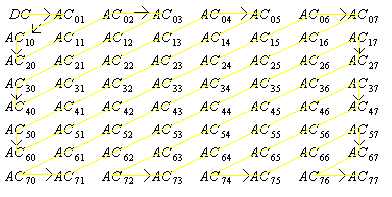
\includegraphics[width=0.5\textwidth]{Billeder/zigzagkoef.png}
%\caption{Nummerering af de transformerede koefficienter.}
%\label{fig:zigzagnummerering}
%\end{figure}
